\section{Testing Environment}
\label{sec:testingEnv}

%% 
%% Leave first page empty
\thispagestyle{empty}

This chapter will describe which tools will be used to run the performance tests in WebRTC, different tools will be used.

\subsection{Stats API}

WebRTC carries a subsection of methods to help developers to access the lower layer network information, this methods return all different types of statistics and performance indicators that we will be using to build our own JavaScript Stats API. When using those statistics we will measure all the congestion KPIs to analyze them.

The method used is the RTCStatsCallback returns a dictionary object (JSON) that has be parsed and manipulated to get the correct indicators, this object returns as many streams as available in a PeerConnection, usually audio and video. This data is provided by the lower layers of the network channel using the RTCP packets that come multiplexed in the RTP stream~\cite{rtpusageIETF}.

The Stats API is the way that WebRTC allows the developer to access different metrics, as this is still in an ongoing discussion the stats report object has not been totally defined and can slightly change, the methods used by the Stats API are available on the W3C editors draft ~\cite{editorWebRTCdraft}. 

We have built a JavaScript tool that uses those stats from the browser to calculate the RTT, throughput and loss rate for the different streams that are being received. Those stats can later be saved into a file or sent as a JSON object to a centralized monitoring system. Our JavaScript grabs any PeerConnection passed through the variable and starts looping an iteration to collect those stats and either plot them or save them into an array for post-processing. 

Figure~\ref{fig:onetooneWifiRTC} shows an example capture of a call between two browsers in two different machines, Mac and Ubuntu, the call was made over Wifi open network with no firewall in the middle but with real traffic. The measures are directly obtained from the Stats API JS file we have built and post-processed using {\it gnuplot}.

 \begin{figure}[h]
  \centering
    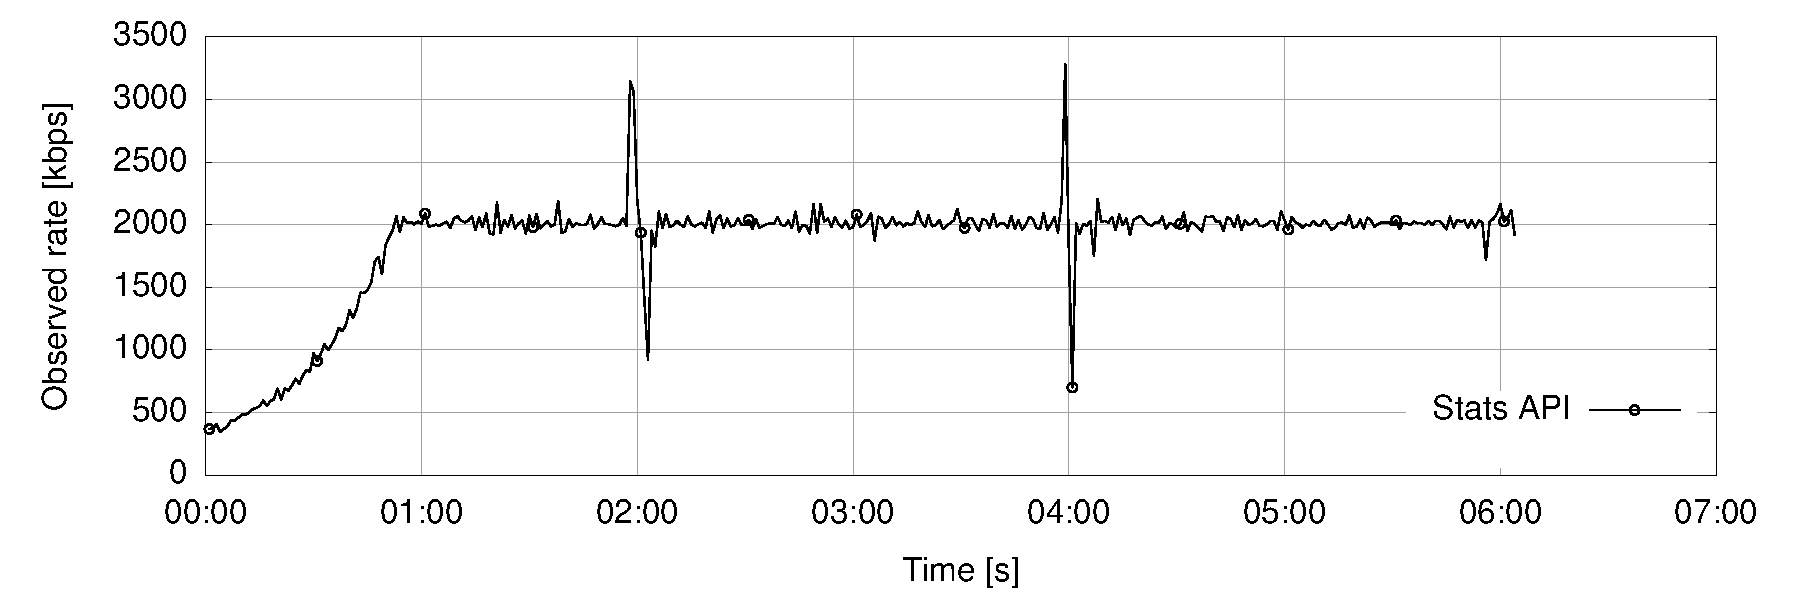
\includegraphics[width=1\textwidth]{./figures/onetooneWifiStatsRTC.pdf}
      \caption[Point-to-point WebRTC video call total throughput graph using Stats API over public WiFi]{Point-to-point WebRTC video call total throughput graph using Stats API over public WiFi.}
	\label{fig:onetooneWifiRTC}
\end{figure}

The previous Figure~\ref{fig:onetooneWifiRTC} considers the global bandwidth of the call, this means that the input/output video and audio are measured together to check how much bandwidth is being consumed over the duration of the call, as it is using RTCP packets for the metrics it takes a while to reach the average rate value. We can then plot all the different streams together to get an idea of how much bandwidth is consuming every stream.

 \begin{figure}[h]
  \centering
    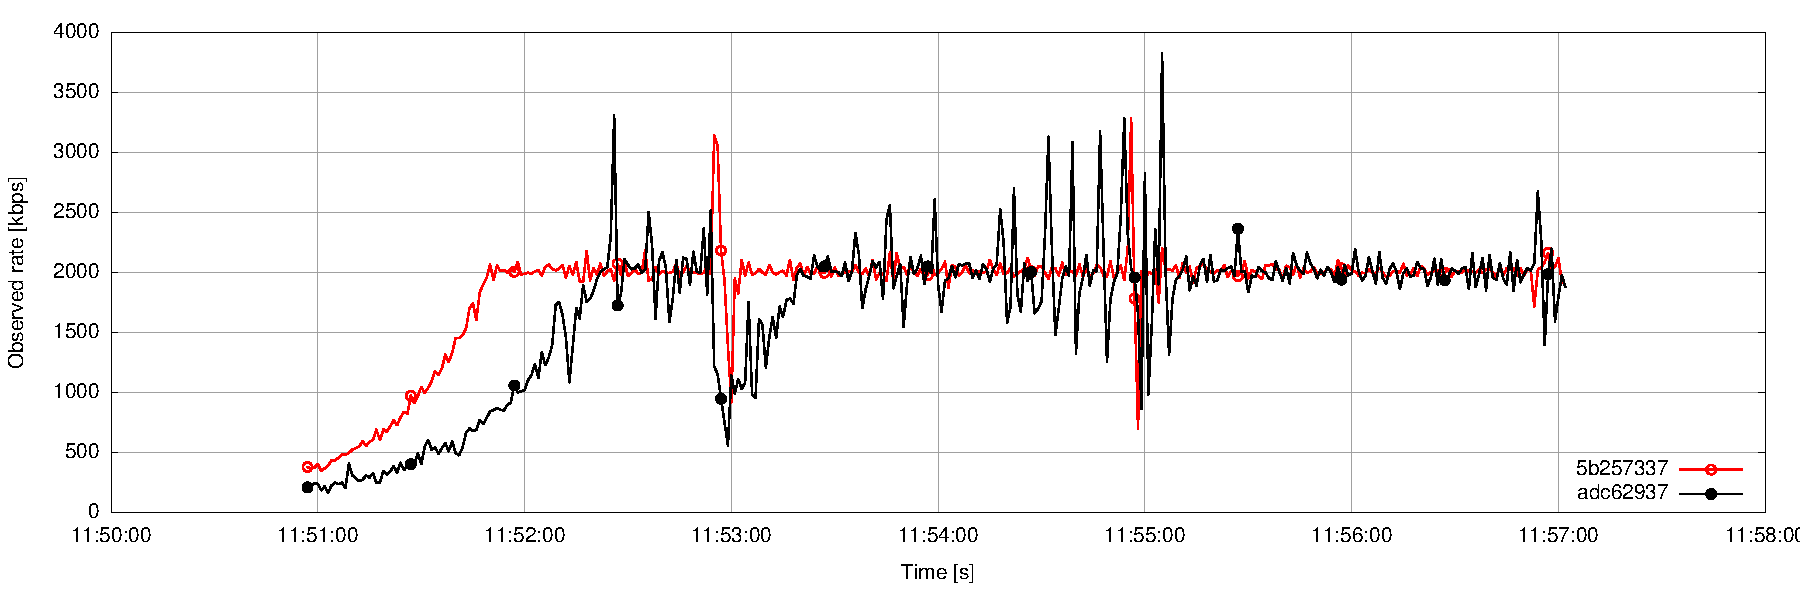
\includegraphics[width=1\textwidth]{./figures/onetooneWiFIStatsVideoStreams.pdf}
      \caption[Point-to-point WebRTC input/output video throughput graph using Stats API over public WiFi]{Point-to-point WebRTC input/output video throughput graph using Stats API over public WiFi.}
	\label{fig:onetooneWifiRTCVideoStreams}
\end{figure}

Figure~\ref{fig:onetooneWifiRTCVideoStreams} shows the two video streams captured from the same machine, one is outgoing the local video stream meanwhile the second stream is the incoming video stream from the other peer. We have built a flexible processing system that allows us to capture and analyze all the possible combinations of streams and metrics. The timing used for the capture is provided by the TimeStamp available on the RTCP. The average bandwidth used in this scenario of point-to-point call in a standard wireless network is around 2000 Kbps per video stream. Both figures are plotted from the same original call.

Our Stats API also provides extra information such as RTT and loss rate, RTT should be provided natively by the WebRTC method but it is possible to calculate it by using the DataChannel provided by the PeerConnection, we are using this channel to send a UNIX TimeStamp object to the other peer and take it back, when the round trip is finished we compare it with the actual millisecond and obtain the total RTT.

 \begin{figure}[h]
  \centering
    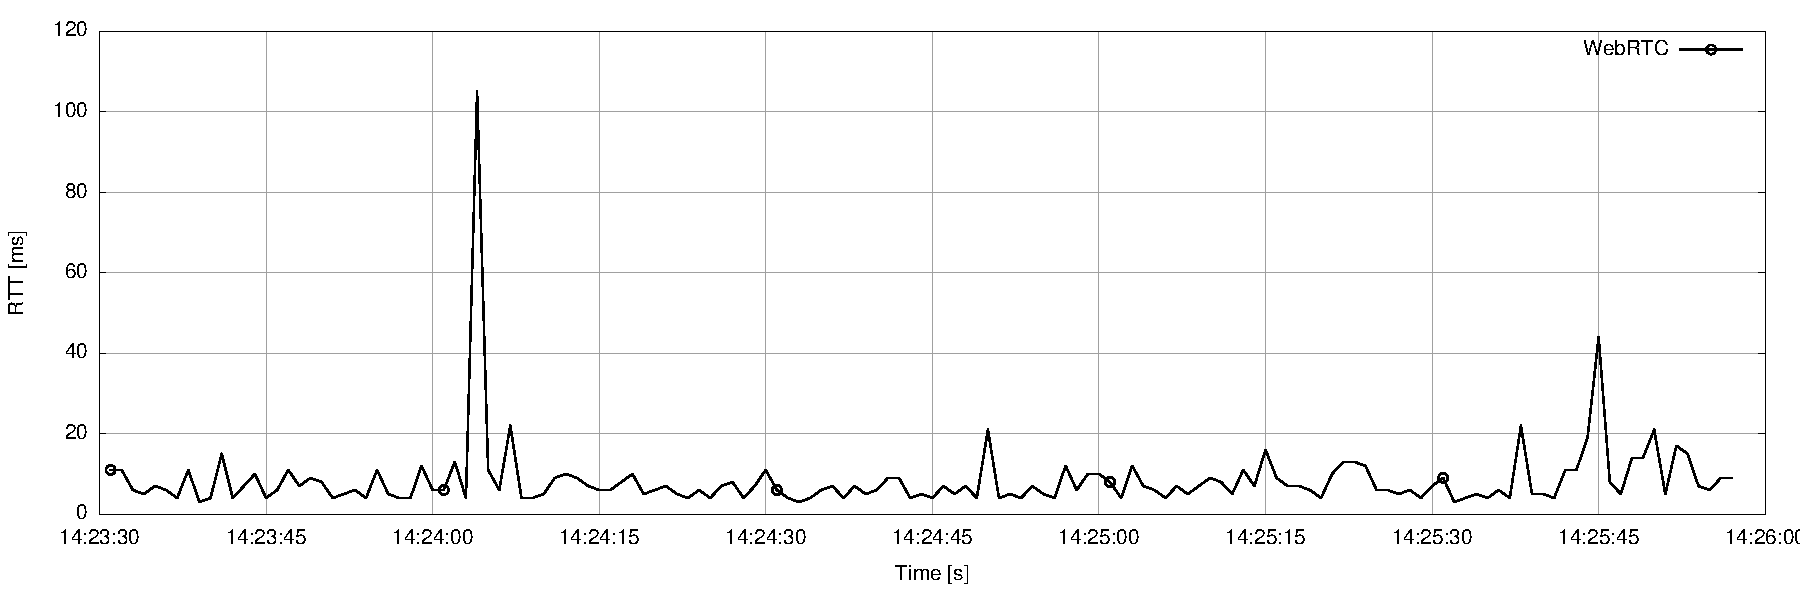
\includegraphics[width=1\textwidth]{./figures/p2prttexample.pdf}
      \caption[Point-to-point WebRTC RTT measure using Stats API over public WiFi]{Point-to-point WebRTC RTT measure using Stats API over public WiFi.}
	\label{fig:p2prttexample}
\end{figure}

Figure~\ref{fig:p2prttexample} represents the capture of a video call between two peers, if we are able to process the JavaScript forwarding function in an optimal way this would led to a precise RTT measurement hack without the need of Stats method.

\subsection{Connection Monitor}

Connection Monitor ({\it ConMon}) is a command line utility that relies on the transport layer and uses TCPDUMP to sniff all the packets that to go a certain interface and port. This application is designed to specifically detect and capture RTP/UDP packets, relies on {\it libcap} for the capture in the network layer. This software detects and saves the header but discards the payload of the packet keeping the information we need for calculating our KPIs.

Typically we will run the PeerConnections between two devices and start capturing those packets by using {\it ConMon}. The PeerConnection will carry real data so the environment for testing will be a precise approach to a real scenario of WebRTC usage.

{\it ConMon} captures will be saved into different files and allow us to plot every stream bandwidth and calculate other parameters such as delay by using some parsing, this will allow us to compare how precise are both way of analyzing WebRTC as {\it ConMon} is working directly over the incoming interface and avoids all the processing that the browser is doing to send the stats to the JavaScript layer. Figure~\ref{fig:onetooneWifiRTCConMon} represents one video stream from the same call as Figure~\ref{fig:onetooneWifiRTC} and~\ref{fig:onetooneWifiRTCVideoStreams} but captured from the {\it ConMon} application.

 \begin{figure}[h]
  \centering
    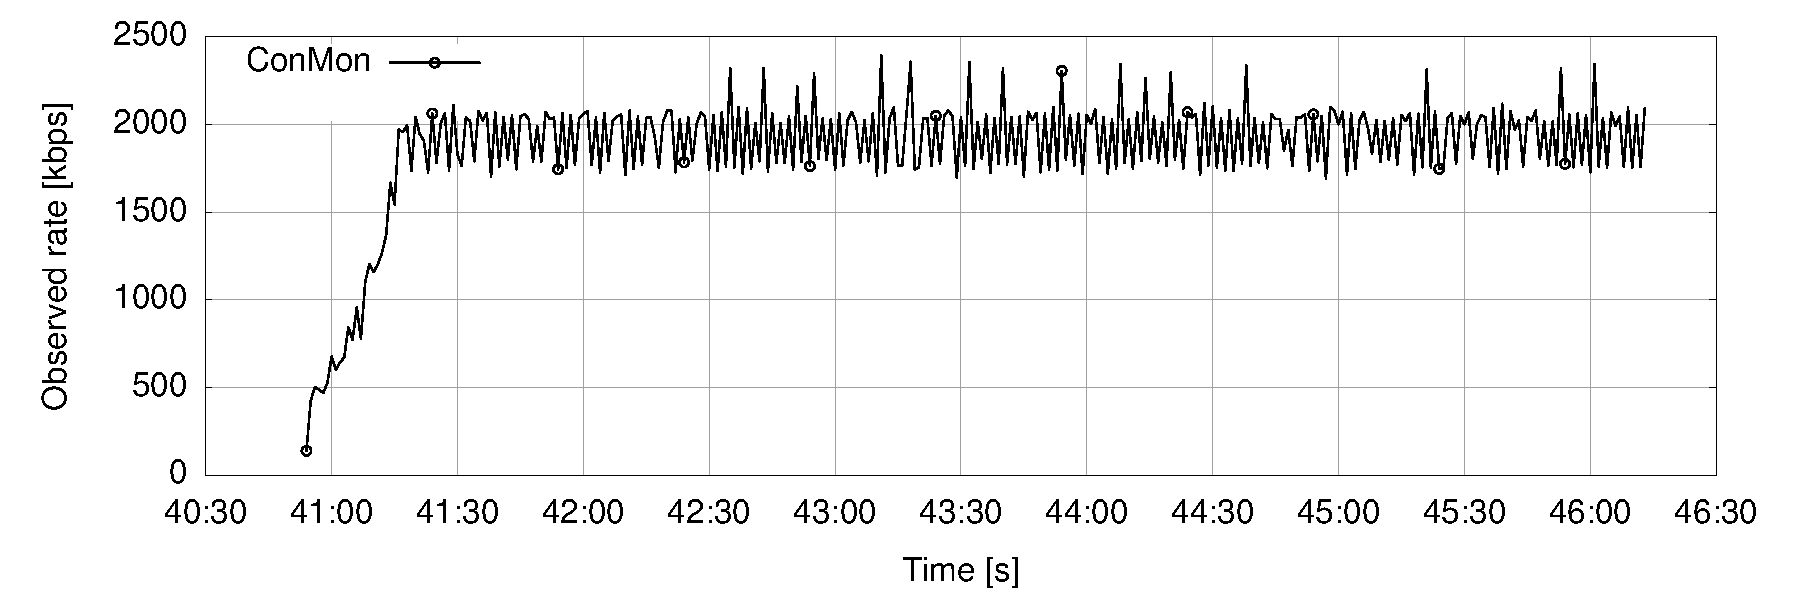
\includegraphics[width=1\textwidth]{./figures/onetooneWiFiConMon.pdf}
      \caption[Point-to-point WebRTC video stream throughput graph using Stats API over public WiFi]{Point-to-point WebRTC video stream throughput graph using Stats API over public WiFi.}
	\label{fig:onetooneWifiRTCConMon}
\end{figure}

The capture from {\it ConMon} will be very accurate capturing all the packets that go through the interface, dumping the values into the output file, this data will then be processed and averaged for every second prior plotting. This processing will lead to some fluctuations on the graph that distort the reality.

\subsection{Dummynet}

To check the performance of WebRTC we will need to modify the status of the network link. This is achieved using {\it Dummynet}, a command line network simulator that allow us to add bandwidth limitations, delays, packet losses and other distortions to the ongoing link. This program will be executed on the computers running the PeerConnections adding those different rules to the interface which is used for the network.

{\it Dummynet} is an standard tool for some Linux distributions and OSX~\cite{dummynetTool}.

\subsection{Analysis of tools}

Both tools will be measuring the same metrics but from different OS layers, this provides us some extra data to be considered in order to see how the our Stats API work and if it is possible to implement some extra features relying on that data for the WebRTC API.

Because of the period needed to measure the results it is possible to have strange behaviors when plotting the results as the information regarding to the next data period can be considered as the previous one. This is an accuracy problem that cannot be approached easily, when looking at the graph is important to see if both peaks (positive and negative) get compensated as this would mean that the data has not been allocated to the current period. This accuracy error is a problem that can be observed when comparing both {\it ConMon} and Stats API capture as the browser will take some time to process the stats and send them to the JavaScript method, this will led to some extra error.

Figure~\ref{fig:p2pincommingStatsConmonWifi} and~\ref{fig:p2poutgoingStatsConmonWifi} plot two video streams being captured from Stats API and {\it ConMon}.

\begin{figure}[h]
	\begin{minipage}{.5\textwidth}
		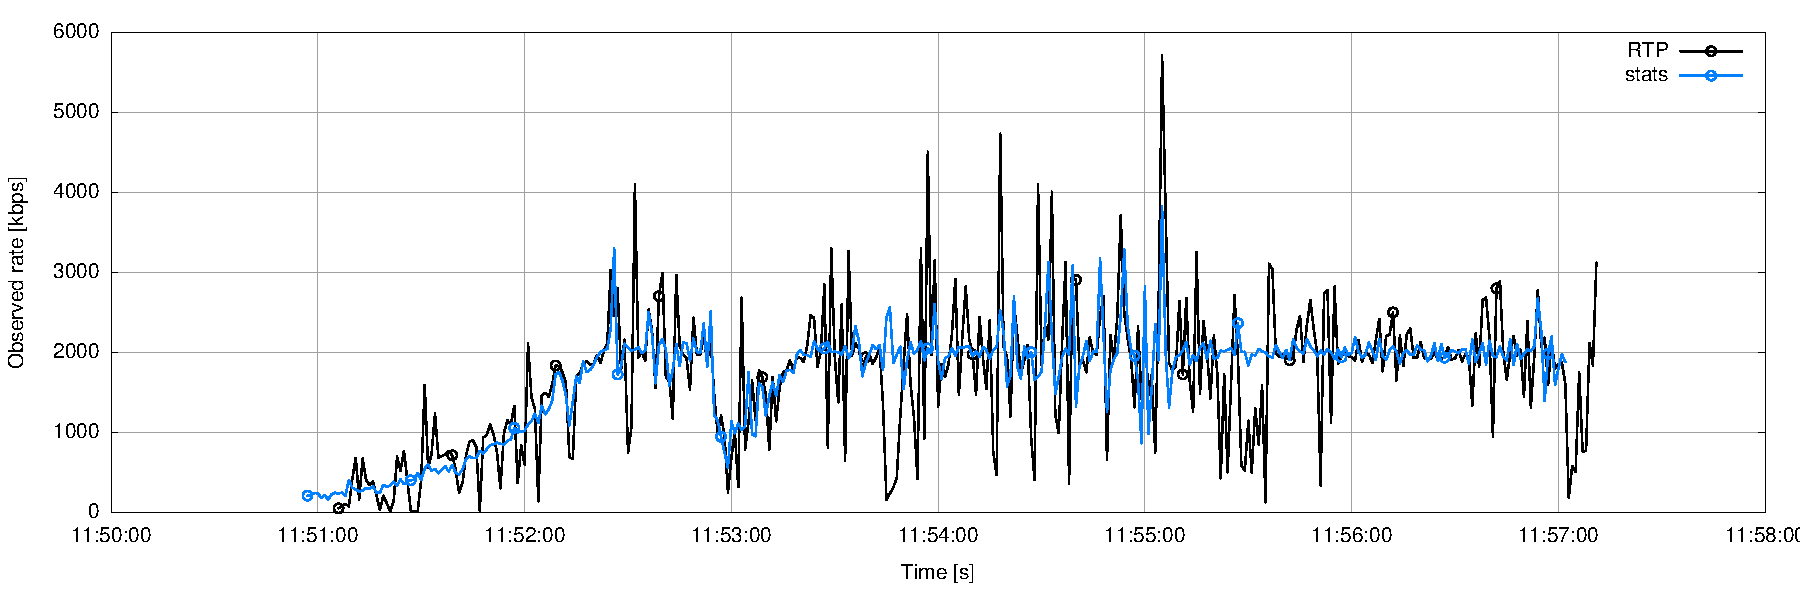
\includegraphics[width=1\textwidth]{./figures/p2pincommingStatsConmonWifi.pdf}
			\caption[P2P incoming video stream comparison between ConMon and Stats API over public WiFi]{P2P incoming video stream comparison between ConMon and Stats API over public WiFi.}
			\label{fig:p2pincommingStatsConmonWifi}
	 \end{minipage}
	 \begin{minipage}{.5\textwidth}
		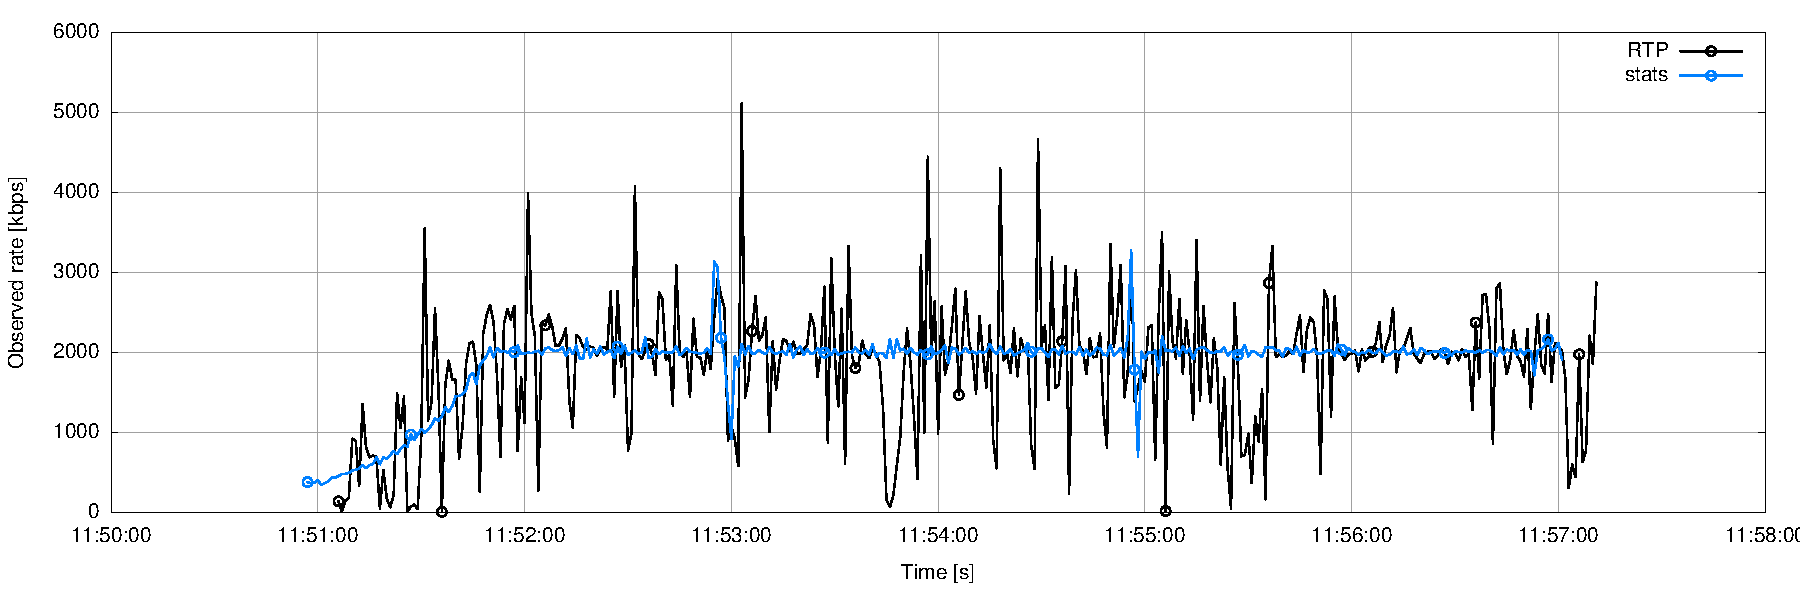
\includegraphics[width=1\textwidth]{./figures/p2poutgoingStatsConmonWifi.pdf}
			\caption[P2P outgoing video stream comparison between ConMon and Stats API over public WiFi]{P2P outgoing video stream comparison between ConMon and Stats API over public WiFi.}
			\label{fig:p2poutgoingStatsConmonWifi}
	 \end{minipage}
\end{figure}

Figure~\ref{fig:p2pincommingStatsConmonWifi} represents the incoming media stream from the other peer, this is why the throughput seems to be so unstable in some parts of the call, consider also that this test was performed using wireless connection without any network conditioner. In Figure~\ref{fig:p2poutgoingStatsConmonWifi} local stream is sent from the peer capturing with {\it ConMon} to the remote peer, the throughput captured using Stats API will be much more stable around the 2000 Kbps.